\documentclass{article}
\usepackage[utf8]{inputenc}
\usepackage[english]{babel}
\usepackage{amsmath}% http://ctan.org/pkg/amsmath
\usepackage{listings}
\usepackage{graphicx}
\usepackage{comment}
\usepackage{float}
\usepackage{biblatex}
\usepackage{lscape}
\usepackage{csquotes}
\usepackage{multirow}
\addbibresource{bibliography.bib}
\usepackage[a4paper,pdftex,bottom=20mm, width=160mm]{geometry} % A4paper margins
\setlength{\parindent}{0pt} % Tar bort indenteringen på paragrafer
\setlength{\parskip}{1em}

\newcommand{\todo}[1]{\textbf{[TODO: #1]}}

\title{
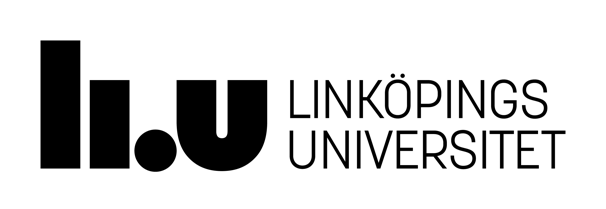
\includegraphics[scale=1.5]{liu_logga.png} \\
\vspace{2.0cm} \textbf{Planning report - The Hive G3 } \\
 \endgraf\rule{\textwidth}{.4pt}
  \large \textbf{TDDE19 Advanced Project Course - AI and Machine Learning}\\
   }


\author{
  \begin{tabular}{ccc}
    Carl Arthur     & Max Eidet       & Oscar Gustafsson \\
    \small carar002 & \small maxei163 & \small oscgu942 \\[1em]
    Jostein Tobias Melaaen & Olle Pettersson & Oskar Schrammel Rask \\
    \small josme010 & \small ollpe910 & \small osksc793 \\
  \end{tabular}
}

\date{\today}

\begin{document}

\maketitle


\newpage
\tableofcontents
\newpage


\section{Introduction}
Small unmanned aerial vehicles (UAVs) are cheap, widely available and hard
to detect, which makes them a growing threat to protected assets such as
infrastructure, bases and public events. Counter-UAS (C-UAS) systems aim to
detect, classify and neutralise such drones \cite{dong2025securing}. One way
to neutralise a drone is with another drone: a defender that finds the
hostile drone with its own sensors, confirms that it is a drone and not, for
example, a bird, and then stops it.

Each step is hard. A small drone far away covers only a few pixels in a
camera image, and at that size it looks much like a bird. Once found, it
moves, so the defender has to steer towards where the target \emph{will} be,
while avoiding trees and the ground.

\newpage
\section{Problem statement} \label{sec:problem_statement}
The project aims to answer two questions:
\begin{enumerate}
    \item How can a hostile drone near a protected asset be detected?
    \item How can the hostile drone be intercepted using a planning-based
          or a reinforcement-learning-based controller?
\end{enumerate}

These are broken down into three questions, each answered by one part of
the system:
\begin{itemize}
    \item \textbf{Surveillance:} how should the defenders be placed and scan
          so that a hostile drone is detected early enough to be intercepted?
          (Section~\ref{sec:base_surveillance})
    \item \textbf{Detection:} at what range, and how reliably, can the
          defenders' cameras detect a small drone and tell it apart from a
          bird? (Section~\ref{sec:detection})
    \item \textbf{Interception:} how much more often, and further from the
          base, does a predictive controller hit the target than pure
          pursuit? (Section~\ref{sec:intercept})
\end{itemize}

Each question is answered by comparing an improved method with a simple
baseline on the same scenarios, using the measures in
Section~\ref{sec:evaluation}. 


\newpage
\section{Setup Overview} \label{sec:setup_overview}
The system is developed and evaluated entirely in simulation, built on three
established open-source tools, so that the project's effort goes into
detection and interception rather than into flight control or physics.

\begin{itemize}
    \item \textbf{PX4} \cite{meier2015px4}
          is the autopilot of every drone in the simulation,
          defenders and hostile drones. It runs as software-in-the-loop,
          the same code that flies real drones, and handles stabilization,
          position control and the motors.
    \item \textbf{Gazebo} \cite{koenig2004gazebo} 
          simulates the world, the
          physics and the sensors: the military camp in a forest, the drones,
          and their cameras.
    \item \textbf{ROS~2} \cite{macenski2022ros2} 
          is the middleware that
          connects our code to PX4 and Gazebo through topics, named streams
          of messages that any program can publish to or read from.
\end{itemize}

Each drone runs its own PX4 instance in the same Gazebo world, with its own
set of ROS~2 topics. Our code reads a drone's position and state from these topics and steers it by continuously sending position, velocity or acceleration setpoints, which PX4 then
flies. Camera images come from Gazebo, and the camera is pointed through PX4. Since Gazebo knows the true position of every drone, each run can also be scored against ground truth, see Section~\ref{sec:evaluation}. The whole setup runs in one Docker container, so every group member has identical software.

Our code is a Python ROS~2 package, built in layers so that the detection
and interception methods do not depend on PX4 directly:

\begin{itemize}
    \item \textbf{Drone layer:} flies one drone through PX4 and points its camera.
    \item \textbf{Swarm layer:} takes off, moves and lands several drones
          together, and places them in formations such as the ring in
          Section~\ref{sec:base_surveillance}.
    \item \textbf{Mission layer:} the components described in the following
          sections. So far it contains the interception part: a tracker that
          estimates the hostile drone's position and velocity, and the
          guidance that steers the defender. Detection and the base station will also be part of this layer.
\end{itemize}



\newpage
\section{Base surveillance} \label{sec:base_surveillance}
While no threat is detected, the defenders watch the sky around the base. They must detect a hostile drone early enough for a defender to intercept it. This section presents different approaches for protecting the base.
\subsection{Baseline: static ring.} The defenders hold fixed, evenly spaced
positions in a ring. Each drone sweeps its outward sector in a fixed tempo by moving the camera, and the images are checked with the detection methods in Section~\ref{sec:detection}.

\subsection{Improvements}
When a defender leaves the ring to intercept, it leaves a gap in the
coverage. The improvement is to close this gap, which can be done in two
ways:
\begin{itemize}
    \item \textbf{Replacement:} a reserve drone is         sent out to take the
          empty position.
    \item \textbf{Redistribution:} the remaining           defenders spread out along
          the ring until they are again evenly spaced, each adjusting its
          position based only on its neighbors, as in
          \cite{kingston2008perimeter}.
\end{itemize}
Both are compared with the static baseline by the coverage lost while a
defender is away from the ring.


\newpage
\section{Drone Detection Using Sensors}
\label{sec:detection}
%Hitta artiklar på hur vi kan detektera drönare.

Thermal camera

detection, finetuna yolo.
gimbal camera, följa dronen.
Finns dataset med fåglar och drönare.
hur kan man mäta performance?
\subsection{YOLO26}
To detect and classify hostile drones, we will use YOLO26 from Ultralytics, the newest version of the YOLO model family \ref{}. YOLO26 looks at an image once and directly outputs where objects are (bounding boxes), what they are (classes), and how confident it is. This makes it fast enough to run in real time.

YOLO26 comes in five sizes, from nano (n) to extra large (x). Larger models are more accurate but need more computing power. Since the detection must eventually run on board the drone, where computing power is limited, we will use the two smallest versions: YOLO26n and YOLO26s.





\newpage
\section{Interception}\label{sec:intercept}
Interception takes over once the detector has classified an object as a
drone with a confidence above a threshold $\tau$ in $k$ consecutive images. The centre of the bounding box is converted into a direction
to the target, using the camera's intrinsic parameters and the gimbal's
orientation, as in \cite{zheng2025mcm}. Two PID controllers turn the gimbal so
that the target stays in the centre of the image, and a Kalman filter smooths
the direction, estimates how fast it turns, and predicts it when the target
is briefly lost. The guidance laws below need only this direction and its
rate of change, not the range, which a single camera measures poorly.

\subsection{Guidance Laws}

\textbf{Baseline: pure pursuit.} The defender flies at full speed towards the
target's current direction, while the gimbal keeps the target in the centre
of the image. This needs only the direction to the target, which one camera
provides. Its weakness is that it always aims at where the target \emph{is},
not where it is going, so against a crossing or turning target it ends up
behind the target and has to chase it.

\textbf{Target system: MPC.} The defender uses the MPC of Zheng et al.\
\cite{zheng2025mcm}. It predicts the target's trajectory over $K$ steps from
its estimated position and velocity, assuming constant velocity, and chooses
the accelerations $\mathbf{u}(k)$ that minimise
\begin{equation}
  J = \sum_{k=1}^{K} \|\mathbf{p}_{\mathrm{exp}}(k) - \mathbf{p}(k)\|^2_{Q}
      + \|\mathbf{u}(k)\|^2_{R},
\end{equation}
where $\mathbf{p}_{\mathrm{exp}}$ is the target's predicted position and
$\mathbf{p}$ the defender's. The problem has an analytical solution; the
first acceleration is sent to PX4 and the problem is solved again at the next
step. Unlike \cite{zheng2025mcm}, who keep an offset around the target to fire
a net, the offset here is zero. Since the hostile drone does not always fly
in a straight line, the constant-velocity prediction is wrong when it turns,
but it is corrected at every step as new estimates arrive; Zheng et al.\
used the same model against a target flying in a circle. The MPC needs the
target's position and velocity, which one camera cannot give. It is therefore
only possible with triangulation from two or more defenders
(Section~\ref{sec:detection}), and is part of the target system.

\subsection{Evaluation}
Metrics are computed by the scenario runner from the true positions in
Gazebo, never from the defender's estimates. The target always flies towards
the base, and a run ends with a \emph{hit} (defender within 1.5 m  of
the target), the \emph{target reaching the base}, the \emph{target is lost}, or a \emph{timeout}. For each run the following are
recorded: 

\begin{itemize}
    \item \textbf{Hit or not:} Whether the defender successfully intercepted the target.
    \item \textbf{Time to hit:} The time elapsed from first detection to interception.
    \item \textbf{Distance to base at hit:} How far the target was from the protected asset when neutralized.
    \item \textbf{Target's closest distance to base:} A measure of how close the threat got before being stopped.
    \item \textbf{Closest distance between defender and target:} Useful for evaluating near-misses in unsuccessful runs.
\end{itemize}

All methods are run on the same seeded scenarios: a target approaching
head-on and crossing at 30, 60 and 90$^\circ$, at increasing speeds
starting at 4~m/s, each 30--50 times. Each method is run both with YOLO detections and with perfect detections from the true position, which
separates errors in guidance from errors in detection.

Since the sensors have not yet been tested, realistic distances and speeds
are not known. Zheng et al.\ \cite{zheng2025mcm} captured a target moving at
4~m/s in 64.7\% of their outdoor attempts. The project aims for a similar
share of hits, and expects proportional navigation to hit more often,
earlier and further from the base than pure pursuit.


\newpage
\section{Baseline System}\label{sec:baseline}
The baseline system is the simplest complete version of the system, built
from the simplest method in each component. Every later method is evaluated
on the same scenarios and compared against it. In each run, a hostile drone spawns at a random location far from the base, with the goal of flying to the military camp in the center of the world. The defender drones are deployed to the formation described in Section~\ref{sec:base_surveillance} and scan the surrounding area with their gimbal cameras. When a defender detects the hostile drone, the detection and classification component decides whether it is a drone. If it is, the defender intercepts it by flying into it.

\newpage
\section{Target System}
%% Oscar Gustafsson

\newpage
\section{System Evaluation}\label{sec:evaluation}
The baseline system and the target system are evaluated with the same
criteria and on the same scenarios, so that their results can be compared
directly. The same criteria are used for every intermediate version, so
that the effect of each improvement can be measured.

\begin{itemize}
    \item \textbf{Mission succeeds} if a defender intercepts the hostile
          drone, that is, comes within 1.5~m of it, while the hostile drone
          is more than $x$~m from its goal.
    \item \textbf{Mission fails} in all other cases: the hostile drone is
          not detected, is first detected within $x$~m of its goal, or is
          not intercepted before it comes within $x$~m of its goal.
    \item \textbf{Mission time} is the time from the hostile drone's spawn
          until the interception. Since all hostile drones spawn at the same
          distance from the base, the mission times of the two systems can
          be compared directly.
\end{itemize}

Each scenario is run 30--50 times with different random spawn locations, all
at the same distance from the base. Fixed random seeds are used, so that
exactly the same runs are repeated for both systems. The results are
reported as the success rate of each system, and as the mean and spread of
the mission times.


\newpage
% Possible final state of the project.
% Include in the planning report with:  \input{final_state}
% Uses only packages the report already loads (amsmath, graphicx, float).

\section{Possible Final State}
\label{sec:final-state}

This section describes a possible end state of the project: what the system
could demonstrate at the end of the course, and how that answers the two
questions in the problem statement. It is a target to steer by rather than a
commitment. All numbers follow from the assumptions in
Section~\ref{sec:assumptions}; when an assumption changes, the derived values
change with it. The work starts small and grows in stages
(Section~\ref{sec:stages}).

\subsection{The Final Demonstration}

In the Gazebo simulation, a ring of $N$ friendly drones patrols at radius $R_p$
around a protected military camp. Each drone carries a wide-angle camera for
short range and a narrow camera on a gimbal that scans the sky outside the
ring. A hostile drone approaches from outside at speed $v_h$. The nearest
friendly drone sees it as a small dark object against the sky. A fast model on
the drone flags the object, and a stronger model at the base station
classifies it as a drone. The base station assigns the friendly drone that can
reach the hostile drone's path in time, while the rest of the ring closes the
gap. The interceptor \emph{locks on}, keeps the target centred in its gimbal
camera, and guides itself to the intercept. Birds appear in the same
scenarios; they are investigated and released, but no hostile drone is let
through. Every run is a seeded scenario that is scored automatically.

\subsection{Assumptions}
\label{sec:assumptions}

Table~\ref{tab:assumptions} lists the assumed values. They are starting
points for the simulation and will be revised as the project progresses.

\begin{table}[H]
\centering
\small
\begin{tabular}{|l|p{0.25\textwidth}|r|p{0.27\textwidth}|}
\hline
\textbf{Symbol} & \textbf{Quantity} & \textbf{Value} & \textbf{Note} \\
\hline
$R_p$ & Perimeter radius & 1000\,m & Ring of friendly drones around the camp \\
$N$ & Number of friendly drones & varies & Derived in Section~\ref{sec:derived} \\
$h$ & Patrol altitude & 50\,m & Same for all friendly drones \\
$h_h$ & Hostile altitude & 20--120\,m & Range the cameras must cover \\
$v_i$ & Interceptor top speed & 12\,m/s & PX4 default for the x500 \\
$v_h$ & Hostile speed & 17\,m/s & Hostile is faster than the interceptor \\
$a$ & Interceptor acceleration & 2\,m/s$^2$ & Used to reach top speed \\
$s$ & Hostile drone size & 0.5\,m & Small quadcopter \\
$p_{\min}$ & Smallest detectable size & 4\,px & Dark object against the sky \\
$\theta_w$, $W_w$ & Wide camera FOV, width & 115$^\circ$, 1280\,px & 3840\,px also considered \\
$\theta_n$, $W_n$, $H_n$ & Narrow camera FOV, image size & 20$^\circ$, 1920$\times$1080\,px & On a gimbal \\
$\Theta_s$ & Sector scanned by the narrow camera & 180$^\circ$ & Outward half only: threats come from outside \\
$t_g$ & Gimbal turn and settle time & 0.5\,s & Per camera position \\
$t_c$ & Image sequence needed to classify & 1.0\,s & Base-station classifier \\
$t_l$ & Radio link and inference latency & 0.1\,s & Drone to base station and back \\
\hline
\end{tabular}
\caption{Assumed values.}
\label{tab:assumptions}
\end{table}

Further simplifying assumptions: the hostile drone flies a straight, radial
path towards the camp at constant speed and altitude; the ring is locally
straight where the hostile drone crosses it; a camera detects the target as
soon as it is at least $p_{\min}$ pixels wide; and there is one hostile drone
at a time.

\subsection{Derived Quantities}
\label{sec:derived}

\textbf{Drone spacing (sparsity).} With $N$ drones evenly spaced on the ring,
the distance between neighbours is
\begin{equation}
  d = \frac{2\pi R_p}{N},
  \label{eq:spacing}
\end{equation}
and a hostile drone that crosses the ring midway between two neighbours passes
at a lateral distance of at most
\begin{equation}
  y_{\max} = \frac{d}{2} = \frac{\pi R_p}{N}
  \label{eq:ymax}
\end{equation}
from the nearest friendly drone.

\textbf{Detection range.} A camera of width $W$ pixels and horizontal field of
view $\theta$ has a focal length, in pixels, of
\begin{equation}
  f = \frac{W/2}{\tan(\theta/2)}.
  \label{eq:focal}
\end{equation}
A target of size $s$ at range $r$ covers $p = f s / r$ pixels, so the
detection range is
\begin{equation}
  r_{\mathrm{det}} = \frac{f\,s}{p_{\min}}.
  \label{eq:rdet}
\end{equation}

\textbf{Coverage without gaps.} Every hostile drone that crosses the ring is
seen if $r_{\mathrm{det}} \geq y_{\max}$, which by Equation~\eqref{eq:ymax}
requires
\begin{equation}
  N \geq \left\lceil \frac{\pi R_p}{r_{\mathrm{det}}} \right\rceil.
  \label{eq:ncoverage}
\end{equation}

\begin{table}[H]
\centering
\small
\begin{tabular}{|l|r|r|r|r|}
\hline
\textbf{Camera} & $f$ (px) & Pixels at 100\,m & $r_{\mathrm{det}}$ & $N$ for no gaps \\
\hline
Wide, 115$^\circ$, 1280\,px & 408 & 2.0 & 51\,m & 62 \\
Wide, 115$^\circ$, 3840\,px & 1223 & 6.1 & 153\,m & 21 \\
Narrow, 20$^\circ$, 1920\,px & 5444 & 27.2 & 681\,m & 5 \\
\hline
\end{tabular}
\caption{Detection range and the number of drones needed for gap-free
coverage, from Equations~\eqref{eq:focal}--\eqref{eq:ncoverage}.}
\label{tab:coverage}
\end{table}

The wide camera alone would need 21--62 drones on a 1\,km ring. The ring is
therefore watched by the narrow cameras, and the wide cameras serve as
short-range backup.

\textbf{Scanning with the narrow camera.} The narrow camera's vertical field of
view is
\begin{equation}
  \theta_v = 2\arctan\!\left(\tan\frac{\theta_n}{2}\cdot\frac{H_n}{W_n}\right)
  \approx 11.3^\circ .
  \label{eq:vfov}
\end{equation}
At range $r_{\mathrm{det}} = 681$\,m, hostile altitudes of 20--120\,m appear
between $-2.5^\circ$ and $+5.9^\circ$ in elevation, which fits within one row
of images. Scanning the outward sector $\Theta_s$ in steps of $\theta_n$ takes
\begin{equation}
  T_{\mathrm{sweep}} = \left\lceil \frac{\Theta_s}{\theta_n} \right\rceil t_g
  = 9 \cdot 0.5\,\mathrm{s} = 4.5\,\mathrm{s},
  \label{eq:sweep}
\end{equation}
during which the hostile drone flies $v_h T_{\mathrm{sweep}} \approx 77$\,m.

\textbf{Time to decide.} In the worst case, the hostile drone enters the
detection range just after the camera has looked past it, so the time from
entering detection range to an assignment is
\begin{equation}
  t_d = T_{\mathrm{sweep}} + t_g + t_c + t_l = 6.1\,\mathrm{s}.
  \label{eq:delay}
\end{equation}

\textbf{Intercept feasibility.} Since $v_h > v_i$, the interceptor cannot catch
the hostile drone from behind; it must reach the hostile drone's path before
the hostile drone gets there. Conservatively, the meeting point is where the
hostile drone crosses the ring. A hostile drone first detected at range
$r_{\mathrm{det}}$ by a drone at lateral distance $y$ reaches the ring after
\begin{equation}
  t_h = \frac{\sqrt{r_{\mathrm{det}}^2 - y^2}}{v_h},
  \label{eq:th}
\end{equation}
and the interceptor reaches the hostile drone's path after
\begin{equation}
  t_i = t_d + \frac{y}{v_i} + \frac{v_i}{2a},
  \label{eq:ti}
\end{equation}
where the last term is the time lost while accelerating to $v_i$. The
intercept is feasible when $t_h \geq t_i$ at the worst case $y = y_{\max}$.

\begin{table}[H]
\centering
\small
\begin{tabular}{|r|r|r|r|r|r|}
\hline
$N$ & $d$ & $y_{\max}$ & $t_h$ & $t_i$ & Margin $t_h - t_i$ \\
\hline
8  & 785\,m & 393\,m & 32.7\,s & 41.8\,s & $-9.1$\,s \\
9  & 698\,m & 349\,m & 34.4\,s & 38.2\,s & $-3.8$\,s \\
10 & 628\,m & 314\,m & 35.5\,s & 35.3\,s & 0.2\,s \\
12 & 524\,m & 262\,m & 37.0\,s & 30.9\,s & 6.0\,s \\
16 & 393\,m & 196\,m & 38.3\,s & 25.5\,s & 12.9\,s \\
20 & 314\,m & 157\,m & 39.0\,s & 22.2\,s & 16.8\,s \\
\hline
\end{tabular}
\caption{Worst-case intercept margin for different numbers of drones, from
Equations~\eqref{eq:spacing}--\eqref{eq:ti} with the narrow camera's detection
range.}
\label{tab:feasibility}
\end{table}

Under these assumptions, the narrow cameras give gap-free coverage from
$N = 5$, but an intercept is only feasible in the worst case from $N = 10$.
The final state therefore assumes about 12 drones, which leaves a margin of
6\,s. Faster scanning, a longer detection range or a faster interceptor reduce
the number of drones needed; the equations above show by how much.

\subsection{Answers to the Problem Statement}

\textbf{Detection.} Detection uses the drones' own cameras. The narrow gimbal
cameras scan the sky outside the ring and detect a 0.5\,m drone at about
680\,m (Table~\ref{tab:coverage}); the wide cameras cover the last 50--150\,m.
When the wide camera reports something, the gimbal turns the narrow camera
towards it for a sharper image (\emph{slew-to-cue}). Classification uses two
tiers: a fast model on the drone, tuned so that it rarely misses a drone, and
a stronger model at the base station that uses short image sequences and
several drones' views. Missing a hostile drone is treated as the worst
outcome, so both tiers favour recall; a false alarm only costs a detour,
during which the target's image grows and the classification improves.

\textbf{Interception.} A planning-based controller serves as the baseline: the
interceptor flies to the predicted meeting point on the hostile drone's path,
then steers with proportional navigation once the camera has locked on. A
controller based on reinforcement learning is trained in a fast, simplified
simulator and runs through the same drone interface, so that the two can be
compared on identical scenarios.

\subsection{System Overview}

Figure~\ref{fig:final-system} shows the system in its final state. The base
station classifies detections and decides which drone does what; each drone
runs its own detection, lock-on and controller, so it can finish an intercept
even if the radio link is lost.

\begin{figure}[H]
\centering
\small
\begin{verbatim}
 BASE STATION
   tracks --> classifier (strong) --> assignment
     ^                                   |
     | image crops + bearings            | roles: patrol /
     |                                   v investigate / intercept
 EACH DRONE
   wide camera + narrow gimbal camera (scanning) --> fast detector
     --> lock-on (detect -> acquire -> locked)
     --> controller (planning or RL) --> PX4 autopilot --> Gazebo
\end{verbatim}
\caption{The system in its final state.}
\label{fig:final-system}
\end{figure}

\subsection{Stages}
\label{sec:stages}

Table~\ref{tab:stages} lists the stages from the current state to the final
one. Later stages only add to earlier ones, so the system works end to end
throughout the project.

\begin{table}[H]
\centering
\small
\begin{tabular}{|p{0.22\textwidth}|p{0.70\textwidth}|}
\hline
\textbf{Stage} & \textbf{What works} \\
\hline
0. Current state &
One interceptor follows one hostile drone at a fixed altitude of 50\,m,
given a noisy estimate of its position, and keeps a safe distance behind it. \\
\hline
1. Lock-on &
A narrow gimbal camera; a simple detector for a dark object against the sky;
a tracker on the camera bearing; a locked state. One hostile drone against
the sky, starting inside the camera's view. \\
\hline
2. Search and intercept &
The narrow camera scans the outward sector; hostile drone at $v_h$ and
interceptor at $v_i$; meeting point on the hostile drone's path and
proportional navigation once locked; a ring of $N$ drones, with the base
station assigning the interceptor. \\
\hline
3. Classification &
Image crops sent to the base station; a classifier over image sequences;
birds as distractors; an \emph{investigate} role; tuning so that no drone is
missed. \\
\hline
4. Wide coverage &
A wide camera on every drone and slew-to-cue; a convolutional neural network
detector that also works against trees and ground. \\
\hline
5. Learned controller (stretch goal) &
An interception policy trained with reinforcement learning, compared with the
planning-based controller; several hostile drones and decoys. \\
\hline
\end{tabular}
\caption{Stages from the current state to the final state.}
\label{tab:stages}
\end{table}

\subsection{Evaluation}

All variants are compared on the same set of seeded scenarios, from easy
(slow, straight approach) to hard (fast, low, evasive, with birds). The main
measure is the number of hostile drones that are missed. Further measures are
the intercept success rate, the time from first detection to lock-on and to
intercept, the number of false pursuits per hour, and the coverage lost while
drones are away from the ring. The derived values in
Section~\ref{sec:derived} are checked against the simulation: for example,
whether the intercept margin in Table~\ref{tab:feasibility} matches the
measured one.

\subsection{Limitations}

Everything runs in simulation; no real drones or sensors are used. The
derived values rest on simplifications: a straight, radial approach at
constant speed, detection as soon as the target is $p_{\min}$ pixels wide, a
clear sky behind the target, and one hostile drone at a time. Real detection
is probabilistic and weaker against clouds, trees or ground. What an intercept
ends with, for example escorting or neutralising the hostile drone, is left
open: the final state ends when the interceptor is locked on and within
intercept distance.





\printbibliography


\end{document}